%----------------------------------------------------------------------------------------
%	PACKAGES AND THEMES
%----------------------------------------------------------------------------------------
\documentclass[aspectratio=169,xcolor=dvipsnames]{beamer}
\usetheme{SimplePlus}

\usepackage[brazilian]{babel}
\usepackage[utf8]{inputenc}
\usepackage{hyperref}
\usepackage{graphicx} % Allows including images
\usepackage{booktabs} % Allows the use of \toprule, \midrule and \bottomrule in tables
% \usepackage[table,dvipsnames]{xcolor}
\usepackage{tikz,tkz-base, tkz-fct,tikz-3dplot,tikz-cd,tkz-tab,tkz-euclide,pgf,pgfplots}
\usepackage{pstricks}
\usepackage{pst-plot}
\usepackage{systeme}
\usepackage{multicol}
\usepackage{lmodern,mathrsfs}
\usepackage{tasks}
\usepackage{float}
\usepackage{array}
\usepackage{multirow}

\pgfplotsset{compat=newest}

%----------------------------------------------------------------------------------------
%	TITLE PAGE
%----------------------------------------------------------------------------------------

\title[short title]{Introdução ao uso de Funções} % The short title appears at the bottom of every slide, the full title is only on the title page
% \subtitle{Subtitle}

\author[Fernando-Jorge] {Fernando Jorge}

\institute[NTU] % Your institution as it will appear on the bottom of every slide, may be shorthand to save space
{
  Escola Estadual Professor Lima Castro
}
\date{\today} % Date, can be changed to a custom date


%----------------------------------------------------------------------------------------
%	PRESENTATION SLIDES
%----------------------------------------------------------------------------------------

\begin{document}

\begin{frame}
    % Print the title page as the first slide
    \titlepage
\end{frame}

\begin{frame}{Sumário}
    % Throughout your presentation, if you choose to use \section{} and \subsection{} commands, these will automatically be printed on this slide as an overview of your presentation
    \tableofcontents
\end{frame}

%------------------------------------------------
\section{Sistemas de coordenadas}
%------------------------------------------------

\begin{frame}{Sistema cartesiano ortogonal de coordenadas}
  \begin{center}
    \begin{tikzpicture}[scale=.6]
      \tkzInit[xmin=-5, xmax=5, xstep=1, ymin=-5, ymax=5, ystep=1]
      \tkzLabelX[orig=false, font=\footnotesize]
      \tkzLabelY[orig=false, font=\footnotesize]
      \tkzDrawXY
      \tkzDefPoint(5,4){P1}
      \tkzDefPoint(-5,3){P2}
      \tkzDefPoint(-4,-4){P3}
      \tkzDefPoint(4,-3){P4}

      \tkzDefPoint(2,0){P5}
      \tkzDefPoint(0,2){P6}

      \tkzDrawPoints[size=3](P1,P2,P3,P4, P5, P6)
      \tkzLabelPoint[above](P1){$P_1(5,4)$}
      \tkzLabelPoint[above](P2){$P_2(-5,3)$}
      \tkzLabelPoint[below](P3){$P_3(-4,-4)$}
      \tkzLabelPoint[below](P4){$P_4(4,-3)$}
      \tkzLabelPoint[above](P5){$P_5(2,0)$}
      \tkzLabelPoint[right](P6){$P_6(0,2)$}
      \tkzPointShowCoord(P1)
      \tkzPointShowCoord(P2)
      \tkzPointShowCoord(P3)
      \tkzPointShowCoord(P4)

      \tkzText[color=cyan](9,-2){Eixo da \textbf{Abscissa} (Ox)}
      \tkzText[color=cyan](-5.1,5.4){Eixo da \textbf{Ordenada} (Oy)}

      \tkzText[color=black](11.2,5){Par Ordenado: $(x,y)$}
      \tkzText[color=black](11.2,4){$P_1 \in Q_1 \implies x > 0 \text{ e } y > 0$}
      \tkzText[color=black](11.2,3){$P_2 \in Q_2 \implies x < 0 \text{ e } y > 0$}
      \tkzText[color=black](11.2,2){$P_3 \in Q_3 \implies x < 0 \text{ e } y < 0$}
      \tkzText[color=black](11.2,1){$P_4 \in Q_4 \implies x > 0 \text{ e } y < 0$}

      \draw[->, >=latex, shorten <=3pt, shorten >= 3pt, color=cyan, thick] (9,-1.8) to [in=-40](5.5,0);
      \draw[->, >=latex, shorten <=3pt, shorten >= 3pt, color=cyan, thick] (-5,4.9) to [out=-34](-0.5,4.5);

      \tkzText[color = red](3,2){$Q_1$}
      \tkzText[color = red](-3,2){$Q_2$}
      \tkzText[color = red](-3,-2){$Q_3$}
      \tkzText[color = red](3,-2){$Q_4$}

      \tkzText[color = black](11,-3){\footnotesize Observação:}
      \tkzText[color = black](11,-4){\footnotesize Em $P_5$, temos $y = 0 \implies P_5 \in Ox$}
      \tkzText[color = black](11,-5){\footnotesize Em $P_6$, temos $x = 0 \implies P_6 \in Oy$}
    \end{tikzpicture}
  \end{center}
\end{frame}

%------------------------------------------------

\begin{frame}{Exercício Resolvido}
  \begin{examples}
    Obter os valores reais de \textit{m} de modo que o ponto $P(2m+1, 3m-6)$ pertença ao quarto quadrante.
  \end{examples}
\end{frame}

%------------------------------------------------

%------------------------------------------------

\begin{frame}{Exercícios Propostos}
  \centering Resolver os exercícios do pdf de Introdução ao estudo de funções, pg: 4
\end{frame}

%------------------------------------------------

\section{O conceito de função}

\begin{frame}{A noção de função}
  Observe o exemplo abaixo:
  \begin{figure}[htb!]
    \centering
    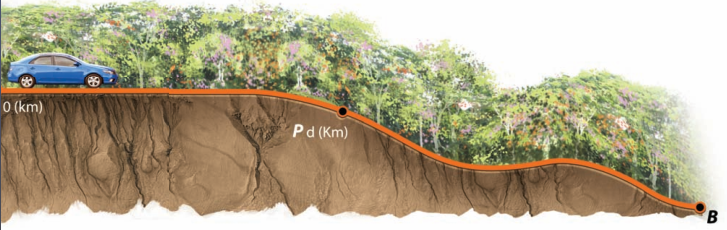
\includegraphics[width=.8\linewidth]{figures/3.png}
  \end{figure}
  Para exemplificar, vamos supor que um automóvel percorra um trecho \textit{AB} de uma estrada à velocidade constante de 
  80 km/h. 

  Que distância terá percorrido o automóvel após 2 horas da partida?
  
\end{frame}

%------------------------------------------------

\begin{frame}{A noção de função}
  \begin{table}
    \begin{tabular}{c c c}
      \toprule
      \textbf{t(hora)} & \textbf{d(quilômetro)} \\
      \midrule
      1      & 80           \\
      2      & 160           \\
      3      & 240           \\
      4      & 320           \\
      \vdots      & \vdots           \\
      \bottomrule
    \end{tabular}
  \end{table}

  Temos que a distância \textit{d} é dada em \textbf{função} do tempo

  Podemos representar a tabela pela expressão matemática:
  \begin{equation*}
    d = 80t
  \end{equation*}
  
\end{frame}

%------------------------------------------------

% \begin{frame}{Multiple Columns}
%     \begin{columns}[c] % The "c" option specifies centered vertical alignment while the "t" option is used for top vertical alignment
%
%         \column{.45\textwidth} % Left column and width
%         \textbf{Heading}
%         \begin{enumerate}
%             \item Statement
%             \item Explanation
%             \item Example
%         \end{enumerate}
%
%         \column{.5\textwidth} % Right column and width
%         Lorem ipsum dolor sit amet, consectetur adipiscing elit. Integer lectus nisl, ultricies in feugiat rutrum, porttitor sit amet augue. Aliquam ut tortor mauris. Sed volutpat ante purus, quis accumsan dolor.
%
%     \end{columns}
% \end{frame}


%------------------------------------------------

\begin{frame}
    \Huge{\centerline{\textbf{Fim}}}
\end{frame}

%----------------------------------------------------------------------------------------

\end{document}
